\documentclass[tikz,border=12pt]{standalone}
\usepackage[T1]{fontenc}
\usepackage{mathpazo}
\usepackage{amsmath,amssymb}
\usetikzlibrary{arrows.meta, positioning, calc, fit, decorations.pathreplacing}

\definecolor{stblue}{HTML}{7B97AD}
\definecolor{rwgold}{HTML}{B8995E}
\definecolor{sage}{HTML}{7A9A7E}
\definecolor{dkbrown}{HTML}{3D3530}
\definecolor{wmgray}{HTML}{7B7067}
\definecolor{cream}{HTML}{F9F6F0}
\definecolor{border}{HTML}{D4C9B8}
\definecolor{terracotta}{HTML}{C47A6A}
\definecolor{lavender}{HTML}{907EA0}
\definecolor{rosefade}{HTML}{B56B6B}

\begin{document}
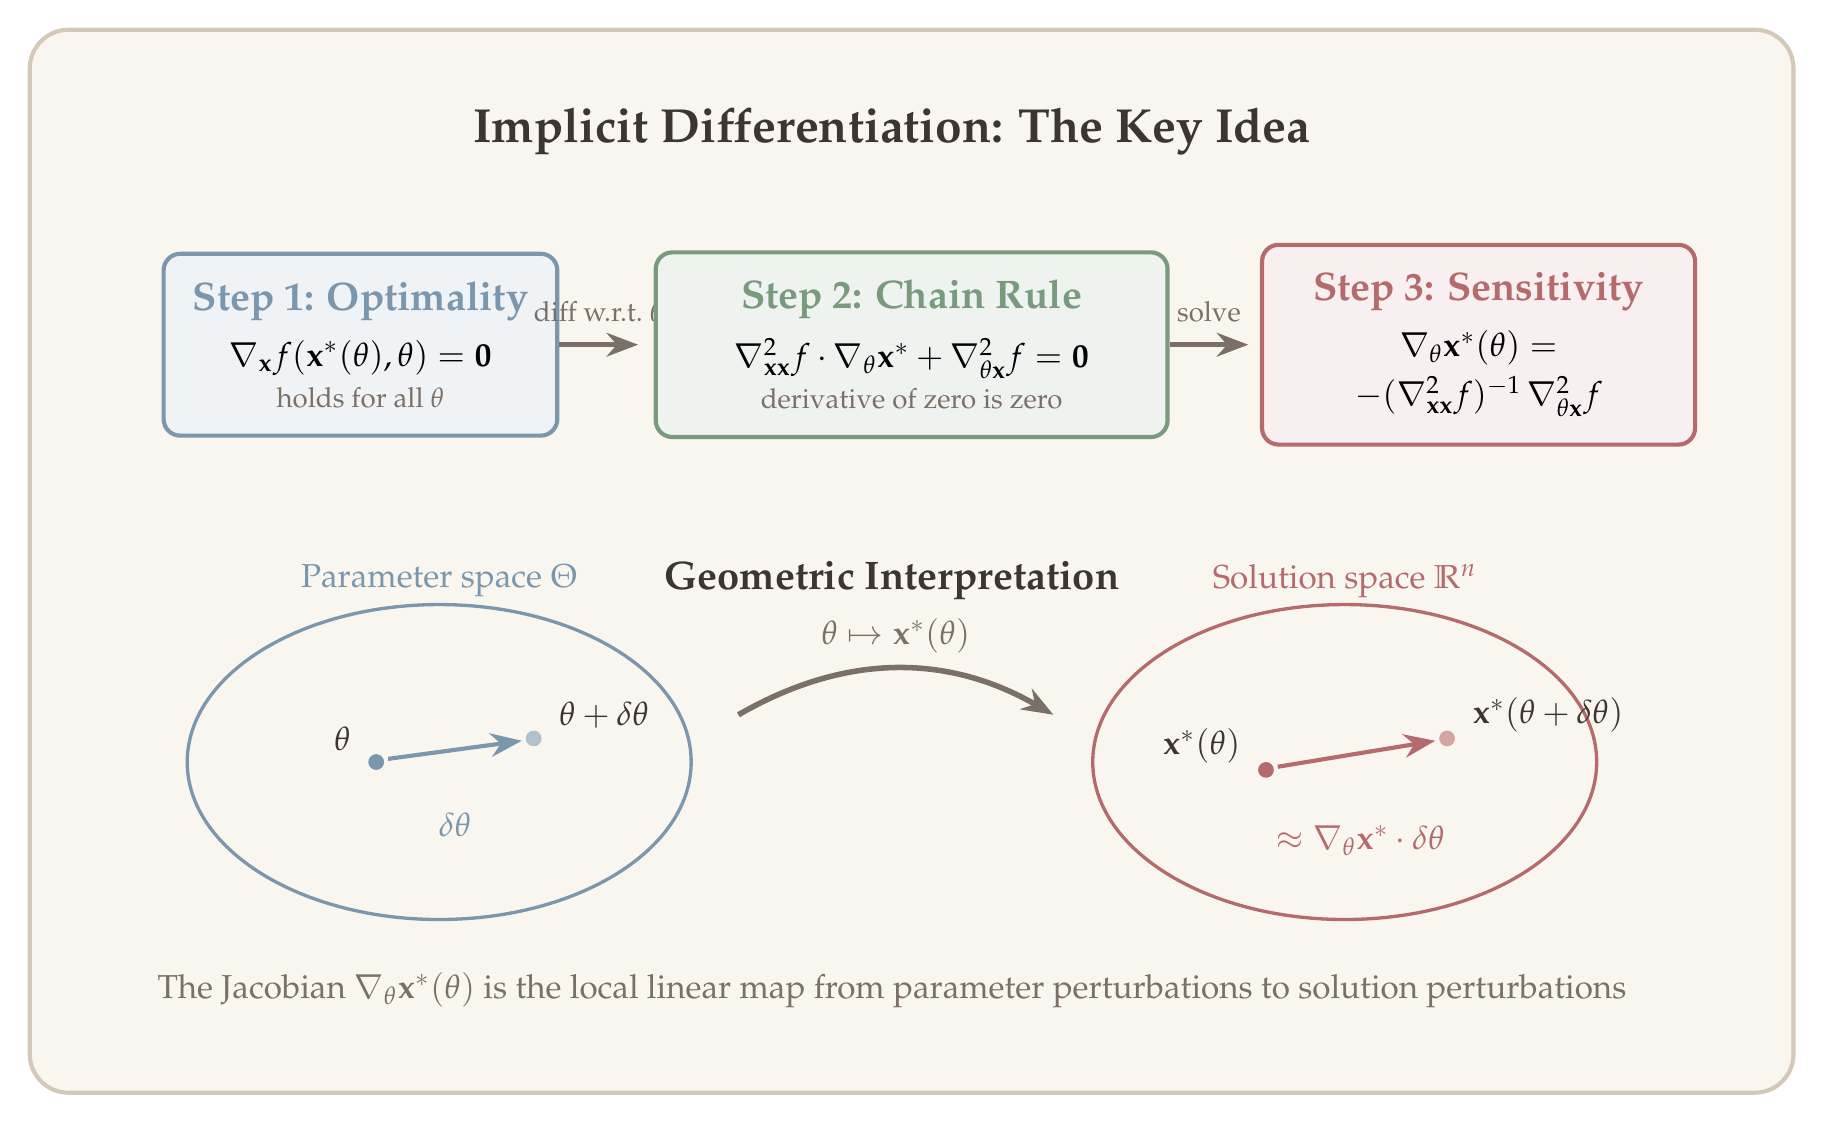
\begin{tikzpicture}[
  >={Stealth[length=4mm, width=3mm]},
  stepbox/.style={rounded corners=6pt, line width=1.5pt, minimum height=2.0cm, align=center, inner sep=10pt},
]

% Background
\fill[cream, rounded corners=14pt] (-1.2,-1.0) rectangle (21.2,12.5);
\draw[border, line width=1.5pt, rounded corners=14pt] (-1.2,-1.0) rectangle (21.2,12.5);

% Title
\node[font=\LARGE\bfseries, text=dkbrown] at (9.75,11.2) {Implicit Differentiation: The Key Idea};

% Step 1: Optimality condition
\node[stepbox, fill=stblue!12, draw=stblue, minimum width=5.0cm] (s1) at (3,8.5) {%
  {\Large\bfseries\color{stblue}Step 1: Optimality}\\[6pt]
  {\large$\nabla_{\mathbf{x}} f(\mathbf{x}^*(\theta), \theta) = \mathbf{0}$}\\[3pt]
  {\normalsize\color{wmgray}holds for all $\theta$}
};

% Arrow 1->2
\draw[wmgray, line width=2pt, ->] (s1.east) -- ++(1.0,0)
  node[midway, above=4pt, font=\normalsize, text=wmgray] {diff w.r.t.\ $\theta$};

% Step 2: Chain Rule
\node[stepbox, fill=sage!12, draw=sage, minimum width=6.5cm] (s2) at (10,8.5) {%
  {\Large\bfseries\color{sage}Step 2: Chain Rule}\\[6pt]
  {\large$\nabla^2_{\mathbf{x}\mathbf{x}} f \cdot \nabla_\theta \mathbf{x}^* + \nabla^2_{\theta\mathbf{x}} f = \mathbf{0}$}\\[3pt]
  {\normalsize\color{wmgray}derivative of zero is zero}
};

% Arrow 2->3
\draw[wmgray, line width=2pt, ->] (s2.east) -- ++(1.0,0)
  node[midway, above=4pt, font=\normalsize, text=wmgray] {solve};

% Step 3: Sensitivity
\node[stepbox, fill=rosefade!10, draw=rosefade, minimum width=5.5cm] (s3) at (17.2,8.5) {%
  {\Large\bfseries\color{rosefade}Step 3: Sensitivity}\\[6pt]
  {\large$\nabla_\theta \mathbf{x}^*(\theta) =$}\\[3pt]
  {\large$-(\nabla^2_{\mathbf{x}\mathbf{x}} f)^{-1}\, \nabla^2_{\theta\mathbf{x}} f$}
};

% --- Geometric interpretation ---
\node[font=\Large\bfseries, text=dkbrown] at (9.75,5.5) {Geometric Interpretation};

% Left: Parameter space
\draw[stblue, line width=1.2pt] (4,3.2) ellipse (3.2 and 2.0);
\node[font=\large, text=stblue] at (4,5.5) {Parameter space $\Theta$};

% theta point
\fill[stblue] (3.2,3.2) circle (0.1);
\node[font=\large, text=dkbrown, anchor=east] at (3.0,3.5) {$\theta$};

% perturbed theta
\fill[stblue!60] (5.2,3.5) circle (0.1);
\node[font=\large, text=dkbrown, anchor=west] at (5.4,3.8) {$\theta + \delta\theta$};

% perturbation arrow
\draw[stblue, line width=1.5pt, ->] (3.35,3.24) -- (5.05,3.47);
\node[font=\large, text=stblue] at (4.2,2.4) {$\delta\theta$};

% Big mapping arrow
\draw[wmgray, line width=2pt, ->] (7.8,3.8) to[out=30, in=150] (11.8,3.8);
\node[font=\large, text=wmgray] at (9.8,4.8) {$\theta \mapsto \mathbf{x}^*(\theta)$};

% Right: Solution space
\draw[rosefade, line width=1.2pt] (15.5,3.2) ellipse (3.2 and 2.0);
\node[font=\large, text=rosefade] at (15.5,5.5) {Solution space $\mathbb{R}^n$};

% x* point
\fill[rosefade] (14.5,3.1) circle (0.1);
\node[font=\large, text=dkbrown, anchor=east] at (14.3,3.4) {$\mathbf{x}^*(\theta)$};

% perturbed x*
\fill[rosefade!60] (16.8,3.5) circle (0.1);
\node[font=\large, text=dkbrown, anchor=west] at (17.0,3.8) {$\mathbf{x}^*(\theta+\delta\theta)$};

% solution perturbation arrow
\draw[rosefade, line width=1.5pt, ->] (14.65,3.14) -- (16.65,3.47);
\node[font=\large, text=rosefade] at (15.7,2.2) {$\approx \nabla_\theta \mathbf{x}^* \cdot \delta\theta$};

% Bottom annotation
\node[font=\large, text=wmgray] at (9.75,0.3)
  {The Jacobian $\nabla_\theta \mathbf{x}^*(\theta)$ is the local linear map from parameter perturbations to solution perturbations};

\end{tikzpicture}
\end{document}
